\documentclass[border=10pt]{standalone}
\usepackage{tkz-fct}
\usepackage{tkz-base}
\usepackage{array}

\begin{document}

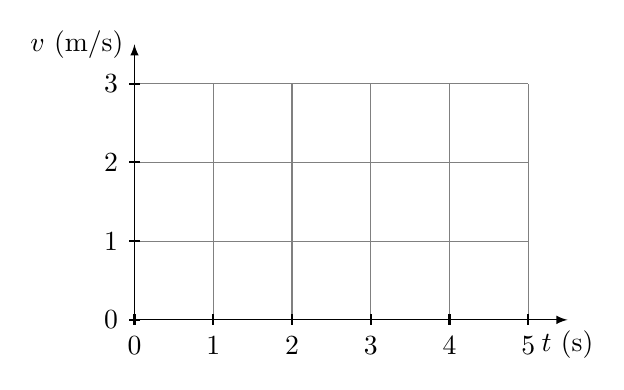
\begin{tikzpicture}
% Tableau en LaTeX standard avec tkz-text

% Repère quadrillé
\begin{scope}
\tkzInit[xmin=0,xmax=5,ymin=0,ymax=3, ystep=1]
\tkzGrid
\tkzDrawX[label = $t$ (s)]
\tkzDrawY[label = $v$ (m/s)]
\tkzLabelXY
\tkzFct[line width=2pt, domain=0:5]{2}
\end{scope}
\end{tikzpicture}

\end{document}
